\documentclass{beamer}
\usetheme{tokitex}

\usepackage{tikz}
\usepackage{graphics}
\usepackage{multirow}
\usepackage{tabto}
\usepackage{xspace}
\usepackage{amsmath}
\usepackage{hyperref}
\usepackage{wrapfig}
\usepackage{mathtools}

\usepackage{tikz}
\usepackage{clrscode3e}
\usepackage{gensymb}

\usepackage[english,bahasa]{babel}
\newtranslation[to=bahasa]{Section}{Bagian}
\newtranslation[to=bahasa]{Subsection}{Subbagian}

\usepackage{listings, lstautogobble}
\usepackage{color}

\definecolor{dkgreen}{rgb}{0,0.6,0}
\definecolor{gray}{rgb}{0.5,0.5,0.5}
\definecolor{mauve}{rgb}{0.58,0,0.82}

\lstset{frame=tb,
  language=c++,
  aboveskip=0mm,
  belowskip=0mm,
  showstringspaces=false,
  columns=fullflexible,
  keepspaces=true,
  basicstyle={\small\ttfamily},
  numbers=none,
  numberstyle=\tiny\color{gray},
  keywordstyle=\color{blue},
  commentstyle=\color{dkgreen},
  stringstyle=\color{mauve},
  breaklines=true,
  breakatwhitespace=true,
  lineskip={-3pt}
}

\usepackage{caption}
\captionsetup[figure]{labelformat=empty}

\newcommand{\progTerm}[1]{\textbf{#1}}
\newcommand{\foreignTerm}[1]{\textit{#1}}
\newcommand{\newTerm}[1]{\alert{\textbf{#1}}}
\newcommand{\emp}[1]{\alert{#1}}
\newcommand{\statement}[1]{"#1"}

\newcommand{\floor}[1]{\lfloor #1 \rfloor}
\newcommand{\ceil}[1]{\lceil #1 \rceil}
\newcommand{\abs}[1]{\left\lvert#1\right\rvert}
\newcommand{\norm}[1]{\left\lVert#1\right\rVert}

% Getting tired of writing \foreignTerm all the time
\newcommand{\farray}{\foreignTerm{array}\xspace}
\newcommand{\fArray}{\foreignTerm{Array}\xspace}
\newcommand{\foverhead}{\foreignTerm{overhead}\xspace}
\newcommand{\fOverhead}{\foreignTerm{Overhead}\xspace}
\newcommand{\fsubarray}{\foreignTerm{subarray}\xspace}
\newcommand{\fSubarray}{\foreignTerm{Subarray}\xspace}
\newcommand{\fbasecase}{\foreignTerm{base case}\xspace}
\newcommand{\fBasecase}{\foreignTerm{Base case}\xspace}
\newcommand{\ftopdown}{\foreignTerm{top-down}\xspace}
\newcommand{\fTopdown}{\foreignTerm{Top-down}\xspace}
\newcommand{\fbottomup}{\foreignTerm{bottom-up}\xspace}
\newcommand{\fBottomup}{\foreignTerm{Bottom-up}\xspace}
\newcommand{\fpruning}{\foreignTerm{pruning}\xspace}
\newcommand{\fPruning}{\foreignTerm{Pruning}\xspace}

\newcommand{\fgraph}{\foreignTerm{graph}\xspace}
\newcommand{\fGraph}{\foreignTerm{Graph}\xspace}
\newcommand{\froot}{\foreignTerm{root}\xspace}
\newcommand{\fRoot}{\foreignTerm{Root}\xspace}
\newcommand{\fnode}{\foreignTerm{node}\xspace}
\newcommand{\fNode}{\foreignTerm{Node}\xspace}
\newcommand{\fedge}{\foreignTerm{edge}\xspace}
\newcommand{\fEdge}{\foreignTerm{Edge}\xspace}
\newcommand{\fcycle}{\foreignTerm{cycle}\xspace}
\newcommand{\fCycle}{\foreignTerm{Cycle}\xspace}
\newcommand{\fdegree}{\foreignTerm{degree}\xspace}
\newcommand{\fDegree}{\foreignTerm{Degree}\xspace}
\newcommand{\fadjacencylist}{\foreignTerm{adjacency list}\xspace}
\newcommand{\fAdjacencylist}{\foreignTerm{Adjacency list}\xspace}
\newcommand{\fadjacencymatrix}{\foreignTerm{adjacency matrix}\xspace}
\newcommand{\fAdjacencymatrix}{\foreignTerm{Adjacency matrix}\xspace}
\newcommand{\fedgelist}{\foreignTerm{edge list}\xspace}
\newcommand{\fEdgelist}{\foreignTerm{Edge list}\xspace}
\newcommand{\flist}{\foreignTerm{list}\xspace}
\newcommand{\fList}{\foreignTerm{List}\xspace}
\newcommand{\fgraphtraversal}{\foreignTerm{graph traversal}\xspace}
\newcommand{\fGraphtraversal}{\foreignTerm{Graph traversal}\xspace}
\newcommand{\ftree}{\foreignTerm{tree}\xspace}
\newcommand{\fTree}{\foreignTerm{Tree}\xspace}
\newcommand{\fsubtree}{\foreignTerm{subtree}\xspace}
\newcommand{\fSubtree}{\foreignTerm{Subtree}\xspace}
\newcommand{\fparent}{\foreignTerm{parent}\xspace}
\newcommand{\fParent}{\foreignTerm{Parent}\xspace}
\newcommand{\fsibling}{\foreignTerm{sibling}\xspace}
\newcommand{\fSibling}{\foreignTerm{Sibling}\xspace}
\newcommand{\fpath}{\foreignTerm{path}\xspace}
\newcommand{\fPath}{\foreignTerm{Path}\xspace}
\newcommand{\fconnectedcomponent}{\foreignTerm{connected component}\xspace}
\newcommand{\fConnectedcomponent}{\foreignTerm{Connected component}\xspace}
\newcommand{\fbridge}{\foreignTerm{bridge}\xspace}
\newcommand{\fBridge}{\foreignTerm{Bridge}\xspace}
\newcommand{\farticulationpoint}{\foreignTerm{articulation point}\xspace}
\newcommand{\fArticulationpoint}{\foreignTerm{Articulation point}\xspace}
\newcommand{\ftreeedge}{\foreignTerm{tree edge}\xspace}
\newcommand{\fTreeedge}{\foreignTerm{Tree edge}\xspace}
\newcommand{\fbackedge}{\foreignTerm{back edge}\xspace}
\newcommand{\fBackedge}{\foreignTerm{Back edge}\xspace}
\newcommand{\fforwardedge}{\foreignTerm{forward edge}\xspace}
\newcommand{\fForwardedge}{\foreignTerm{Forward edge}\xspace}
\newcommand{\fcrossedge}{\foreignTerm{cross edge}\xspace}
\newcommand{\fCrossedge}{\foreignTerm{Cross edge}\xspace}
\newcommand{\fdiscoverytime}{\foreignTerm{discovery time}\xspace}
\newcommand{\fDiscoverytime}{\foreignTerm{Discovery time}\xspace}
\newcommand{\flowlink}{\foreignTerm{low link}\xspace}
\newcommand{\fLowlink}{\foreignTerm{Low link}\xspace}
\newcommand{\fstack}{\foreignTerm{stack}\xspace}
\newcommand{\fStack}{\foreignTerm{Stack}\xspace}
\newcommand{\for}{\foreignTerm{or}\xspace}
\newcommand{\fOr}{\foreignTerm{Or}\xspace}
\newcommand{\fand}{\foreignTerm{and}\xspace}
\newcommand{\fAnd}{\foreignTerm{And}\xspace}
\newcommand{\fcentroid}{\foreignTerm{centroid}\xspace}
\newcommand{\fCentroid}{\foreignTerm{Centroid}\xspace}

\newcommand{\fDivideAndConquer}{\foreignTerm{Divide and conquer}\xspace}
\newcommand{\fdivideAndConquer}{\foreignTerm{divide and conquer}\xspace}
\newcommand{\fMergeSort}{\foreignTerm{Merge sort}\xspace}
\newcommand{\fmergeSort}{\foreignTerm{merge sort}\xspace}
\newcommand{\fQuickSort}{\foreignTerm{Quicksort}\xspace}
\newcommand{\fquickSort}{\foreignTerm{quicksort}\xspace}
\newcommand{\fpivot}{\foreignTerm{pivot}\xspace}
\newcommand{\fPivot}{\foreignTerm{Pivot}\xspace}
\newcommand{\fbruteForce}{\foreignTerm{brute force}\xspace}
\newcommand{\fBruteForce}{\foreignTerm{Brute force}\xspace}
\newcommand{\fCompleteSearch}{\foreignTerm{complete search}\xspace}
\newcommand{\fExhaustiveSearch}{\foreignTerm{exhaustive search}\xspace}
\newcommand{\fbinarySearch}{\foreignTerm{binary search}\xspace}
\newcommand{\fBinarySearch}{\foreignTerm{Binary search}\xspace}
\newcommand{\fternarySearch}{\foreignTerm{ternary search}\xspace}
\newcommand{\fTernarySearch}{\foreignTerm{Ternary search}\xspace}
\newcommand{\funimodal}{\foreignTerm{unimodal}\xspace}
\newcommand{\fUnimodal}{\foreignTerm{Unimodal}\xspace}
\newcommand{\fGreedy}{\foreignTerm{Greedy}\xspace}
\newcommand{\fgreedy}{\foreignTerm{greedy}\xspace}
\newcommand{\fgreedyChoice}{\foreignTerm{greedy choice}\xspace}
\newcommand{\fGreedyChoice}{\foreignTerm{Greedy choice}\xspace}

\newcommand{\fdp}{\foreignTerm{dynamic programming}\xspace}
\newcommand{\fDp}{\foreignTerm{Dynamic programming}\xspace}
\newcommand{\fbitmask}{\foreignTerm{bitmask}\xspace}
\newcommand{\fBitmask}{\foreignTerm{Bitmask}\xspace}
\newcommand{\fstate}{\foreignTerm{state}\xspace}
\newcommand{\fState}{\foreignTerm{State}\xspace}
\newcommand{\fsubmask}{\foreignTerm{submask}\xspace}
\newcommand{\fSubmask}{\foreignTerm{Submask}\xspace}

\newcommand{\pheap}{\foreignTerm{heap}\xspace}
\newcommand{\pHeap}{\foreignTerm{Heap}\xspace}
\newcommand{\pBinaryHeap}{\foreignTerm{Binary Heap}\xspace}
\newcommand{\pbinaryHeap}{\foreignTerm{binary heap}\xspace}
\newcommand{\pHeapsort}{\foreignTerm{Heapsort}\xspace}
\newcommand{\pheapsort}{\foreignTerm{heapsort}\xspace}
\newcommand{\pdjs}{\foreignTerm{disjoint set}\xspace}
\newcommand{\pDjs}{\foreignTerm{Disjoint set}\xspace}

\newcommand{\fdotProduct}{\foreignTerm{dot product}\xspace}
\newcommand{\fDotProduct}{\foreignTerm{Dot product}\xspace}
\newcommand{\fcrossProduct}{\foreignTerm{cross product}\xspace}
\newcommand{\fCrossProduct}{\foreignTerm{Cross product}\xspace}
\newcommand{\fconvexHull}{\foreignTerm{convex hull}\xspace}
\newcommand{\fConvexHull}{\foreignTerm{Convex hull}\xspace}
\newcommand{\fgrahamScan}{\foreignTerm{graham scan}\xspace}
\newcommand{\fGrahamScan}{\foreignTerm{Graham scan}\xspace}
\newcommand{\flineSweep}{\foreignTerm{line sweep}\xspace}
\newcommand{\fLineSweep}{\foreignTerm{Line sweep}\xspace}

\newcommand{\fset}{\foreignTerm{set}\xspace}
\newcommand{\fSet}{\foreignTerm{Set}\xspace}
\newcommand{\fprefixSum}{\foreignTerm{prefix sum}\xspace}
\newcommand{\fPrefixSum}{\foreignTerm{Prefix sum}\xspace}
\newcommand{\ffenwickTree}{\foreignTerm{fenwick tree}\xspace}
\newcommand{\fFenwickTree}{\foreignTerm{Fenwick tree}\xspace}
\newcommand{\frangeSumQuery}{\foreignTerm{range sum query}\xspace}
\newcommand{\fRangeSumQuery}{\foreignTerm{Range sum query}\xspace}
\newcommand{\fquery}{\foreignTerm{query}\xspace}
\newcommand{\fQuery}{\foreignTerm{Query}\xspace}
\newcommand{\fsegmentTree}{\foreignTerm{segment tree}\xspace}
\newcommand{\fSegmentTree}{\foreignTerm{Segment tree}\xspace}
\newcommand{\fbinaryTree}{\foreignTerm{binary tree}\xspace}
\newcommand{\fBinaryTree}{\foreignTerm{Binary tree}\xspace}
\newcommand{\flazyPropagation}{\foreignTerm{lazy propagation}\xspace}
\newcommand{\fLazyPropagation}{\foreignTerm{Lazy propagation}\xspace}
\newcommand{\fsparseTable}{\foreignTerm{sparse table}\xspace}
\newcommand{\fSparseTable}{\foreignTerm{Sparse table}\xspace}

\newcommand{\ftrail}{\foreignTerm{trail}\xspace}
\newcommand{\fTrail}{\foreignTerm{Trail}\xspace}
\newcommand{\feulerTour}{\foreignTerm{euler tour}\xspace}
\newcommand{\fEulerTour}{\foreignTerm{Euler tour}\xspace}
\newcommand{\feulerTourTree}{\foreignTerm{euler tour tree}\xspace}
\newcommand{\fEulerTourTree}{\foreignTerm{Euler tour tree}\xspace}

\newcommand{\fmaxflow}{\foreignTerm{maximum flow}\xspace}
\newcommand{\fMaxflow}{\foreignTerm{Maximum flow}\xspace}
\newcommand{\fmincut}{\foreignTerm{minimum cut}\xspace}
\newcommand{\fMincut}{\foreignTerm{Minimum cut}\xspace}
\newcommand{\fflow}{\foreignTerm{flow}\xspace}
\newcommand{\fFlow}{\foreignTerm{Flow}\xspace}
\newcommand{\fsource}{\foreignTerm{source}\xspace}
\newcommand{\fSource}{\foreignTerm{Source}\xspace}
\newcommand{\fsink}{\foreignTerm{sink}\xspace}
\newcommand{\fSink}{\foreignTerm{Sink}\xspace}
\newcommand{\fbackEdge}{\foreignTerm{back-edge}\xspace}
\newcommand{\fBackEdge}{\foreignTerm{Back-edge}\xspace}
\newcommand{\fresidualCapacity}{\foreignTerm{residual capacity}\xspace}
\newcommand{\fResidualCapacity}{\foreignTerm{Residual capacity}\xspace}
\newcommand{\fbottleneck}{\foreignTerm{bottleneck}\xspace}
\newcommand{\fBottleneck}{\foreignTerm{Bottleneck}\xspace}
\newcommand{\faugmentingPath}{\foreignTerm{augmenting path}\xspace}
\newcommand{\fAugmentingPath}{\foreignTerm{Augmenting path}\xspace}


\title{Struktur Data Lanjutan}
\author{Tim Olimpiade Komputer Indonesia}
\date{}
\lstset{escapeinside={<@}{@>}}

\begin{document}

\begin{frame}
\titlepage
\end{frame}

\begin{frame}
\frametitle{Pendahuluan}
Melalui dokumen ini, kalian akan:
\begin{itemize}
  \item Memahami penggunaan C++ set/map
  \item Memahami konsep Fenwick Tree
  \item Memahami konsep Segment Tree
  \item Memahami konsep Sparse Table
\end{itemize}
\end{frame}

\begin{frame}[fragile]
\frametitle{C++ set}
\begin{itemize}
  \item Pada C++ STL (Standard Template Library), terdapat tipe data \lstinline{std::set<T>} yang dapat digunakan untuk menyimpan sebuah himpunan (\fset) \lstinline{T}.
  \begin{itemize}
    \item Sebagai contoh, \lstinline{set<int>} merupakan himpunan \lstinline{int}.
  \end{itemize}
  \item Untuk menggunakan tipe data ini, kita harus menambahkan \lstinline{include <set>}.
  \item Pada umumnya, \lstinline{set} akan menyimpan objek secara terurut menaik.
  \begin{itemize}
    \item Perilaku ini dapat diubah menggunakan \foreignTerm{custom comparator}. Sebagai contoh, pada C++11:
\begin{lstlisting}
auto cmp = [](int a, int b) { ... };
set<int, decltype(cmp)> s(cmp);
\end{lstlisting}
  \end{itemize}
  \item \lstinline{set} diimplementasikan menggunakan \foreignTerm{self balancing binary tree}\xspace, yang akan dibahas pada beberapa materi selanjutnya.
\end{itemize}
\end{frame}

\begin{frame}
\frametitle{Operasi C++ set}
\begin{itemize}
  \item Beberapa fungsi/operasi umum yang sering digunakan pada C++ \lstinline{set}.
  \begin{itemize}
    \item \lstinline{set::insert(x)} menambahkan elemen \lstinline{x} pada \lstinline{set} dalam waktu $O(\log N)$.
    \item \lstinline{set::erase(x)} menghapus elemen \lstinline{x} pada \lstinline{set} dalam waktu $O(\log N)$.
    \item \lstinline{set::size()} mengembalikan banyaknya elemen pada \lstinline{set} dalam waktu $O(1)$.
    \item \lstinline{set::count(x)} mengembalikan banyaknya elemen $x$ pada \lstinline{set} dalam waktu $O(\log N)$ (antara $0$ atau $1$).
    \item \lstinline{set::clear()} menghapus seluruh elemen \lstinline{set} dalam waktu $O(N)$.
  \end{itemize}
  dengan $N$ adalah banyaknya elemen pada \lstinline{set}.
\end{itemize}
\end{frame}

\begin{frame}
\frametitle{Set Iterator}
\begin{itemize}
  \item \lstinline{set<int>::iterator} adalah tipe data penunjuk sebuah elemen pada \lstinline{set}.
  \begin{itemize}
    \item Sebagai contoh, operasi \lstinline{set<int>::iterator it = s.begin();} akan membuat iterator \lstinline{it} menunjuk pada elemen pertama pada himpunan \lstinline{s} (jika \lstinline{s} tidak kosong).
    \item Kemudian operasi \lstinline{it++} akan membuat iterator \lstinline{it} menunjuk pada elemen kedua pada himpunan \lstinline{s} (jika \lstinline{s} berisi setidaknya dua bilangan).
    \item Untuk mendapatkan elemen yang ditunjuk, kita dapat menggunakan \lstinline{*it}.
  \end{itemize}
\end{itemize}
\end{frame}

\begin{frame}
\frametitle{Set Iterator (lanj.)}
\begin{itemize}
  \item Beberapa fungsi/operasi umum yang sering digunakan pada C++ \lstinline{set} yang mengembalikan \lstinline{set<int>::iterator} dalam waktu $O(\log N)$.
  \begin{itemize}
    \item \lstinline{set::lower_bound(x)} mengembalikan penunjuk elemen terkecil yang tidak lebih kecil dari \lstinline{x} dalam waktu $O(\log N)$. Jika tidak ada elemen yang memenuhi, maka \lstinline{set::lower_bound(x)} akan mengembalikan \lstinline{set::end()}.
    \item \lstinline{set::upper_bound(x)} mengembalikan penunjuk elemen terkecil yang lebih besar dari \lstinline{x} dalam waktu $O(\log N)$. Jika tidak ada elemen yang memenuhi, maka \lstinline{set::upper_bound(x)} akan mengembalikan \lstinline{set::end()}.
    \item \lstinline{set::find(x)} mengembalikan penunjuk elemen yang bernilai \lstinline{x} dalam waktu $O(\log N)$. Jika tidak ada elemen yang memenuhi, maka \lstinline{set::find(x)} akan mengembalikan \lstinline{set::end()}.
  \end{itemize}
\end{itemize}
\end{frame}

\begin{frame}
\frametitle{Operasi C++ multiset}
\begin{itemize}
  \item C++ \lstinline{std::multiset<T>} merupakan tipe data yang mirip dengan \lstinline{set} namun dapat menyimpan beberapa elemen yang sama.
  \item Beberapa perbedaan antara C++ \lstinline{multiset} dan \lstinline{set}
  \begin{itemize}
    \item \lstinline{multiset::count(x)} dapat mengembalikan bilangan bulat lebih besar dari $1$.
    \item \lstinline{multiset::erase(x)} menghapus seluruh elemen \lstinline{x} pada \lstinline{multiset}. Jika kita ingin menghapus hanya satu elemen \lstinline{x}, gunakan \lstinline{multiset::erase(multiset::find(x))}.
  \end{itemize}
\end{itemize}
\end{frame}

\begin{frame}
\frametitle{C++ map}
\begin{itemize}
  \item C++ \lstinline{std::map<K, V>} merupakan tipe data yang digunakan untuk menyimpan pemetaan dari tipe data \lstinline{K} ke tipe data \lstinline{V}.
  \begin{itemize}
    \item Sebagai contoh, \lstinline{map<string, int>} merupakan pemetaan dari \lstinline{string} ke \lstinline{int}.
    \item Contoh penggunaan tipe data ini adalah untuk menyimpan pemetaan dari nama murid ke nilai ujian, dan mengakses nilai ujian seorang murid dalam waktu cepat.
  \end{itemize}
  \item Untuk menggunakan tipe data ini, kita harus menambahkan \lstinline{include <map>}.
  \item \lstinline{map} juga diimplementasikan menggunakan \foreignTerm{self balancing binary tree}\xspace.
\end{itemize}
\end{frame}

\begin{frame}
\frametitle{Operasi C++ map}
\begin{itemize}
  \item Misalkan kita memiliki \lstinline{map<K, V> myMap;}.
  \item Beberapa fungsi/operasi umum yang sering digunakan pada C++ \lstinline{map}.
  \begin{itemize}
    \item \lstinline{myMap[k]} mengakses nilai pemetaan \lstinline{k} dalam waktu $O(\log N)$.
    \item \lstinline{myMap[k] = v} menentukan atau mengganti pemetaan dari \lstinline{k} menjadi ke \lstinline{v} dalam waktu $O(\log N)$.
    \item \lstinline{myMap.erase(k)} menghapus nilai pemetaan $k$ dalam waktu $O(\log N)$.
    \item \lstinline{myMap.count(k)} mengembalikan $1$ jika terdapat nilai pemetaan $k$, atau $0$ jika tidak, dalam waktu $O(\log N)$.
    \item \lstinline{myMap.clear()} menghapus seluruh pemetaan dalam waktu $O(N)$.
  \end{itemize}
  dengan $N$ adalah banyaknya elemen pada \lstinline{myMap}.
\end{itemize}
\end{frame}

\begin{frame}
\frametitle{Persoalan Range Sum Query}
\begin{itemize}
  \item Persoalan \newTerm{Range Sum Query} adalah persoalan menghitung jumlah elemen berurutan pada sebuah \farray $A$ berukuran $N$.
  \begin{itemize}
    \item Pada umumnya, diberikan $Q$ pertanyaan yang merepresentasikan sebuah \fsubarray.
  \end{itemize}
  \item Jika \farray yang diberikan tidak dapat berubah, persoalan ini dapat diselesaikan menggunakan \fprefixSum yang menjawab satu pertanyaan dalam waktu $O(1)$.
  \item Jika \farray yang diberikan dapat berubah, persoalan ini dapat diselesaikan menggunakan \ffenwickTree yang menjawab satu pertanyaan dalam waktu $O(\log N)$ dan mengganti satu elemen \farray dalam waktu $O(\log N)$.
\end{itemize}
\end{frame}

\begin{frame}
\frametitle{Fenwick Tree}
\begin{itemize}
  \item \newTerm{Fenwick Tree} (sering disebut juga \newTerm{Binary Indexed Tree}) adalah data struktur yang menyimpan sebuah \farray berukuran $N$ dengan indeks $1$ sampai $N$ dengan setiap elemennya menyimpan jumlah elemen berurutan pada \farray $A$.
  \begin{itemize}
    \item $BIT[j]$ menyimpan jumlah elemen $\sum_{i=j - LSBIT(j) + 1}^{j} A[i]$, dengan $LSBIT(j)$ adalah nilai dari \lstinline{j & (-j)} pada C++. Sebagai contoh,
    \begin{itemize}
      \item $LSBIT(1) = 1, BIT[1] = A[1]$,
      \item $LSBIT(2) = 2, BIT[2] = A[1] + A[2]$,
      \item $LSBIT(3) = 1, BIT[3] = A[3]$,
      \item $LSBIT(4) = 4, BIT[4] = A[1] + A[2] + A[3] + A[4]$, dan
      \item $LSBIT(6) = 2, BIT[6] = A[5] + A[6]$.
    \end{itemize}
  \end{itemize}
\end{itemize}
\end{frame}

\begin{frame}
\frametitle{Fenwick Tree (lanj.)}
\begin{itemize}
  \item Dengan \ffenwickTree, kita dapat menghitung nilai $\sum_{i=1}^{x} A[i]$ dalam $O(\log N)$.
  \begin{itemize}
    \item Sebagai contoh, menghitung nilai $A[1] + A[2] + A[3] + A[4] + A[5] + A[6]$ dapat disederhanakan menjadi $(A[1] + A[2] + A[3] + A[4]) + (A[5] + A[6]) = BIT[4] + BIT[6]$.
  \end{itemize}
  \item Secara umum, $\sum_{i=1}^{x}$ dapat dihitung menggunakan rumus berikut:
  \begin{itemize}
    \item $0$, jika $x = 0$,
    \item $BIT[x] + \sum_{i=1}^{x - LSBIT(x)}$, jika $x > 0$.
  \end{itemize}
\end{itemize}
\end{frame}

\begin{frame}
\frametitle{Fenwick Tree (lanj.)}
\begin{itemize}
  \item Jika nilai $A[i]$ berubah, maka kita harus memperbaharui semua nilai $BIT[j]$ yang memenuhi $j - LSBIT(j) < i \leq j$. Terdapat $O(\log N)$ nilai yang harus diperbaharui.
  \begin{itemize}
    \item Sebagai contoh, jika nilai $A[5]$ berubah, maka kita harus memperbaharui nilai $BIT[5], BIT[6], BIT[8], BIT[16], \cdots$.
  \end{itemize}
  \item Secara umum, jika nilai $A[i]$ berubah menjadi $A[i] + \delta$, kita dapat memanggil fungsi \lstinline{update(i)} yang melakukan hal berikut jika $i \leq N$:
  \begin{itemize}
    \item Perbaharui nilai $BIT[i]$ menjadi $BIT[i] + \delta$.
    \item Panggil fungsi \lstinline{update(i + LSBIT(i))}.
  \end{itemize}
\end{itemize}
\end{frame}

\begin{frame}
\frametitle{Segment Tree}
\begin{itemize}
  \item \newTerm{Segment Tree} merupakan struktur data alternatif untuk menyelesaikan persoalan \frangeSumQuery.
  \item \fSegmentTree merupakan \fbinaryTree. Tiap \fnode memiliki informasi nilai dari suatu rentang atau segmen. Ukuran segmen dari suatu \fnode pada \fsegmentTree merupakan gabungan segmen dari anak-anaknya.
\end{itemize}
\end{frame}

\begin{frame}
\frametitle{Ilustrasi Segment Tree}
\begin{itemize}
  \item Misalkan kita memiliki \farray berukuran $N$. \fSegmentTree dari \farray tersebut memiliki $O(\log N)$ tingkat.
  \item Secara keseluruhan, terdapat maksimal $2N$ segmen. Kompleksitas memori dari \fsegmentTree adalah $O(N)$.
  \item Untuk memudahkan implementasi, kita nomori setiap \fnode pada \fsegmentTree. \fRoot dari \ftree ini dinomori $1$, dengan anak kiri dan kanan dari \fnode $x$ dinomori $2x$ dan $2x + 1$ secara berurutan.
\end{itemize}
\end{frame}

\begin{frame}
\frametitle{Ilustrasi Segment Tree (lanj.)}
\begin{itemize}
  \item Sebagai contoh, berikut merupakan bentuk \fsegmentTree untuk menghitung \frangeSumQuery dari \farray $[5, -3, 2, 1, 4, 4, -1, 6]$.
  \item Tiap \fnode memiliki informasi jumlah dari segmen yang dilingkupinya.
\end{itemize}
\begin{center}
  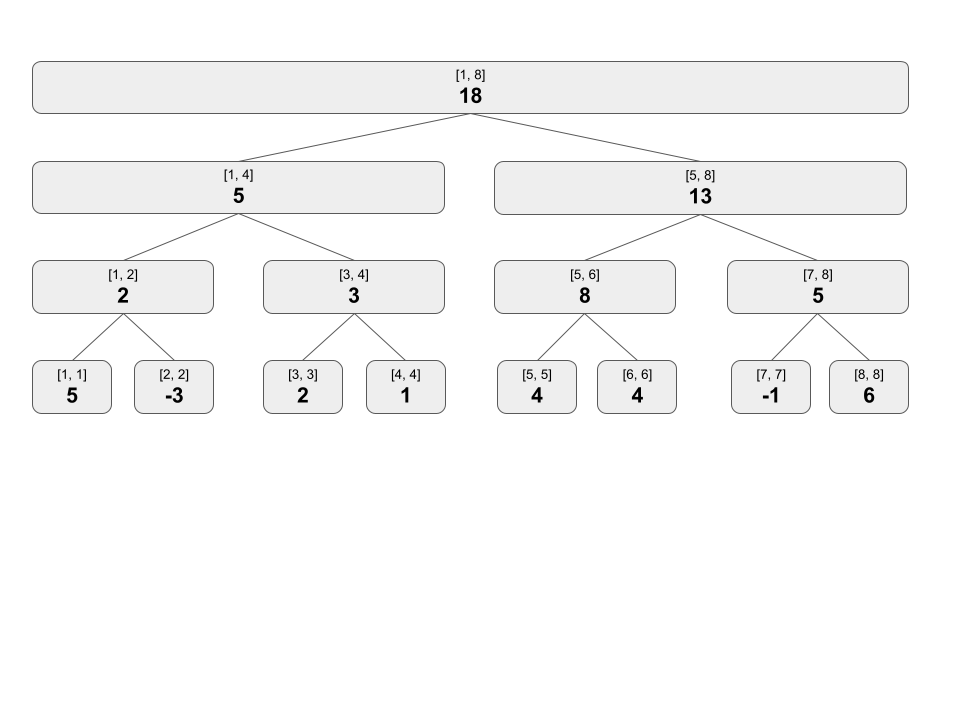
\includegraphics[width=10cm]{asset/segtree-init.png}
\end{center}
\end{frame}

\begin{frame}[fragile]
\frametitle{Inisiasi Segment Tree}
\begin{itemize}
  \item Berikut adalah contoh kode untuk menginisiasi \fsegmentTree untuk menghitung \frangeSumQuery.
  \item $MAXA$ dihitung dengan $2^{\lceil \log_{2}N \rceil + 1}$.
\end{itemize}
\begin{lstlisting}
int st[MAXA];         // informasi jumlah segmen

void build(int idx, int l, int r) {
  if (l == r) {
    st[idx] = val[l];
    return;
  }

  int mid = (l + r) / 2;
  build(idx * 2    , l, mid); // rekursif ke kiri
  build(idx * 2 + 1, mid + 1, r); // rekursif ke kanan
  
  st[idx] = st[idx * 2] + st[idx * 2 + 1];
}

...
bulid(1, 1, N); // pemanggilan awal
\end{lstlisting}
\end{frame}

\begin{frame}
\frametitle{Query pada Segment Tree}
\begin{itemize}
  \item Untuk mendapatkan jumlah dari interval $L$ sampai $R$, kita cukup menjumlahkan segmen-segmen yang membentuk interval $L$ sampai $R$. Terdapat paling banyak $O(\log N)$ segmen yang harus dijumlahkan.
  \item Berikut adalah ilustrasi untuk menjumlahkan elemen dari indeks $2$ sampai $6$.
\end{itemize}
\begin{center}
  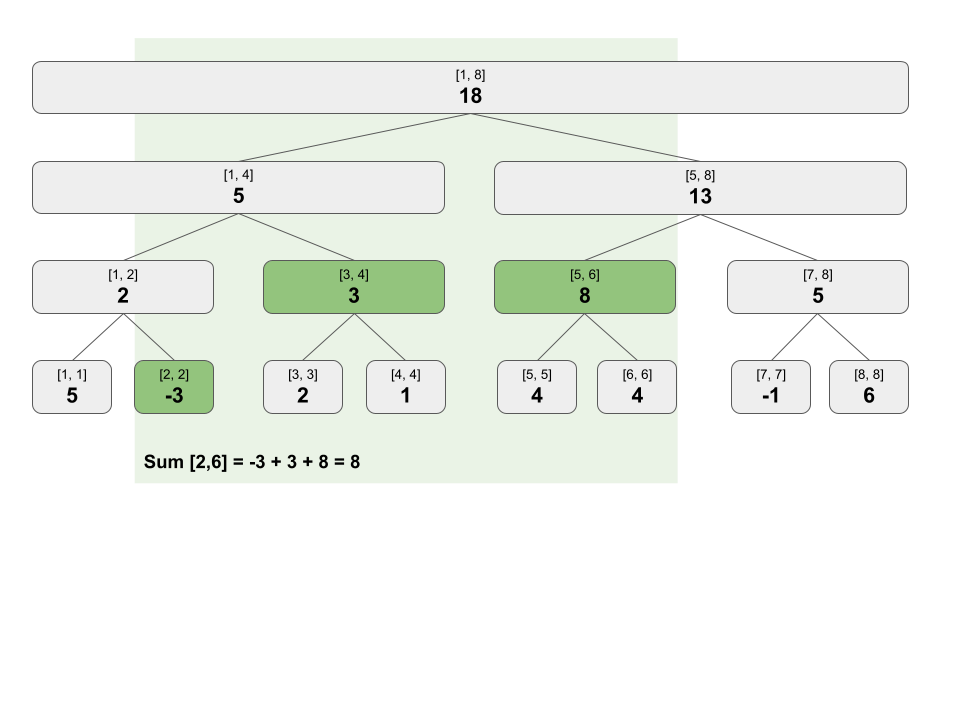
\includegraphics[width=10cm]{asset/segtree-sum.png}
\end{center}
\end{frame}

\begin{frame}[fragile]
\frametitle{Kode Query pada Segment Tree}
\begin{itemize}
  \item \fQuery dapat dicapai dengan melakukan penjelajahan \fsegmentTree dari segmen terbesar, dan berhenti ketika kita berada di segmen yang sepenuhnya di dalam segmen yang ingin dijumlahkan.
\end{itemize}
\begin{lstlisting}
int query(int idx, int l, int r, int x, int y) {
  if (x > r || y < l)
    // node ini berada di luar segmen query
    return 0;

  if (x <= l && r <= y)
    // node ini berada di dalam segmen query
    return st[idx];
  
  int mid = (l + r) / 2;
  return query(idx * 2    , l, mid, x, y) +
         query(idx * 2 + 1, mid + 1, r, x, y);
}
\end{lstlisting}
\end{frame}

\begin{frame}
\frametitle{Single Point Update pada Segment Tree}
\begin{itemize}
  \item Untuk memperbaharui nilai elemen di suatu indeks, kita cukup memperbaharui nilai seluruh segmen yang melingkupi indeks tersebut.
  \item Kompleksitas untuk tiap perbaharuan adalah $O(\log N)$.
  \item Berikut adalah ilustrasi menambahkan nilai $2$ pada indeks $4$.
\end{itemize}
\begin{center}
  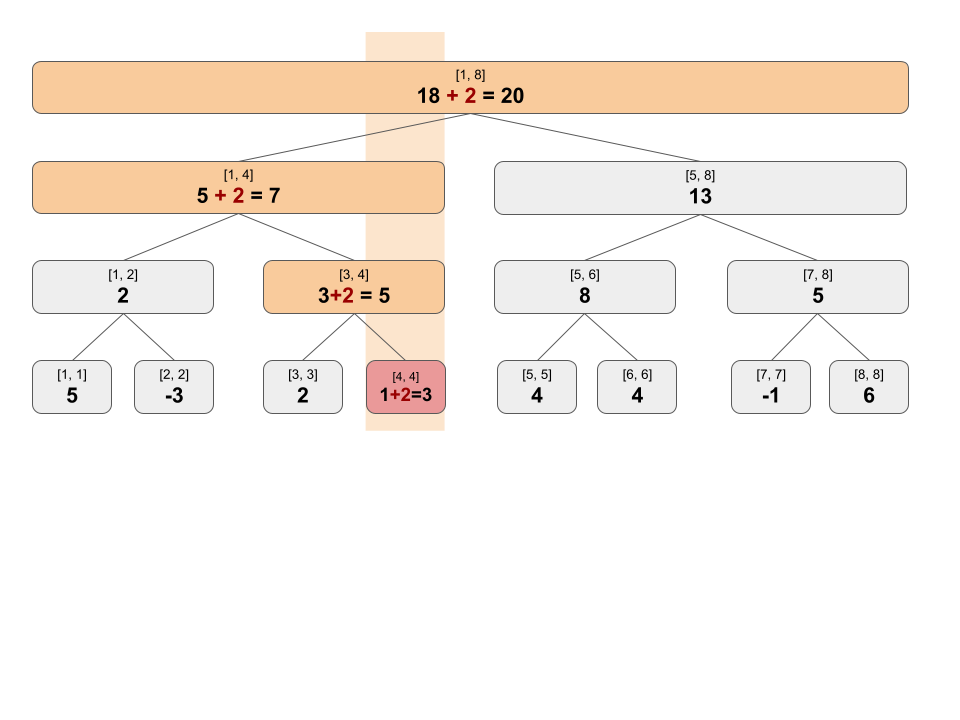
\includegraphics[width=10cm]{asset/segtree-update.png}
\end{center}
\end{frame}

\begin{frame}[fragile]
\frametitle{Kode Single Point Update}
\begin{itemize}
  \item Berikut adalah contoh kode jika kita ingin menambahkan nilai $v$ pada suatu indeks $x$.
\end{itemize}
\begin{lstlisting}
void update(int idx, int l, int r, int x, int v) {
  // perbaharui jumlah nilai pada segmen ini
  st[idx] += v;     

  if (l == r) 
    // node tanpa anak
    return;

  // kunjungi anak yang benar
  int mid = (l + r) / 2;
  if (x <= mid) 
    update(idx * 2    , l, mid, x, v);
  else 
    update(idx * 2 + 1, mid + 1, r, x, v);
}
\end{lstlisting}
\end{frame}

\begin{frame}
\frametitle{Range Update pada Segment Tree}
\begin{itemize}
  \item Bagaimana jika kita harus memperbaharui beberapa elemen sekaligus dalam suatu segmen?
  \item Misalnya, untuk suatu segmen $[A,B]$, tambahkan nilainya dengan $v$.
  \item Kita bisa melakukan penjelajahan pada \fsegmentTree, dan berhenti di daun yang termasuk dari segmen.
  \item Namun, kasus terburuknya adalah jika kita harus memperbaharui keseluruhan range, sehingga kita harus memperbaharui keseluruhan $O(N)$ \fnode pada \fsegmentTree.
\end{itemize}
\end{frame}

\begin{frame}
\frametitle{Lazy Propagation}
\begin{itemize}
  \item Agar dapat memperbaharui segmen dengan lebih efisien, kita cukup berhenti pada segmen yang sudah sepenuhnya di dalam segmen yang ingin diperbaharui.
  \item Karena kita berhenti di segmen $X$, kita sebenarnya belum memperbaharui informasi pada segmen-segmen yang merupakan anak dari $X$.
  \item Karena itu, kita perlu menyiapkan informasi tambahan yang menyatakan perbaharuan yang belum diselesaikan. Informasi ini akan dipropagasi nanti ketika kita melakukan penjelajahan di segmen tersebut.
  \item Teknik ini disebut dengan \newTerm{Lazy Propagation}.
\end{itemize}
\end{frame}

\begin{frame}
\frametitle{Ilustrasi Lazy Propagation}
\begin{itemize}
  \item Berikut adalah ilustrasi dari \flazyPropagation untuk menambahkan nilai $2$ ke indeks $3$ sampai $5$.
\end{itemize}
\begin{center}
  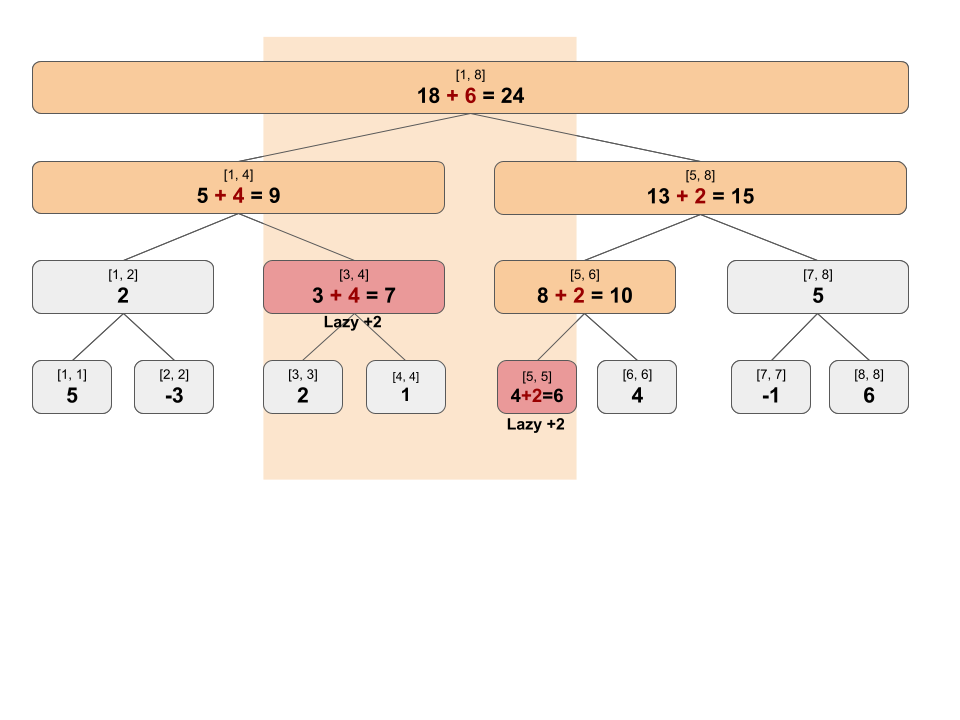
\includegraphics[width=10cm]{asset/segtree-update-lazy.png}
\end{center}
\end{frame}

\begin{frame}[fragile]
\frametitle{Kode Lazy Propagation}
\begin{itemize}
  \item Berikut adalah kode untuk melakukan \flazyPropagation.
\end{itemize}
\begin{lstlisting}
void update(int idx, int l, int r, int x, int y, int v) {
  if (x < r || l > y) return; // berhenti jika di luar
                              // segmen
  if (x <= l && r <= y) {
    // perbaharui jumlah segmen ini
    st[idx] += (r - l + 1) * v;     
    // perbaharui nilai "lazy" segmen ini
    lazy[idx] += v;                 
    return;
  }
  
  int mid = (l + r) / 2;

  propagate(idx, l, r);
  update(idx * 2    , l, mid, x, y, v);
  update(idx * 2 + 1, mid + 1, r, x, y, v);
  
  st[idx] = st[idx * 2] + st[idx * 2 + 1];
}
\end{lstlisting}
\end{frame}

\begin{frame}[fragile]
\frametitle{Kode Propagasi}
\begin{itemize}
  \item Fungsi tambahan \lstinline{propagate} adalah untuk meneruskan perbaharuan yang belum dieksekusi ke anak segmen.
\end{itemize}
\begin{lstlisting}
void propagate(int idx, int l, int r) {
  // hanya perlu dilakukan jika nilai "lazy" tidak 0
  if (lazy[idx]) { 
    int mid = (l + r)/2, lc = idx * 2, rc = idx * 2 + 1;
    // propagasi ke anak kiri
    lazy[lc] += lazy[idx];
    st[lc] += (mid - l + 1) * lazy[idx]; 
    // propagasi ke anak kanan
    lazy[rc] += lazy[idx];
    st[rc] += (r - mid) * lazy[idx];

    lazy[idx] = 0; // bersihkan nilai "lazy"
  }
}
\end{lstlisting}
\end{frame}

\begin{frame}[fragile]
\frametitle{Query dengan Lazy Propagation}
\begin{itemize}
  \item \fQuery pada \fsegmentTree yang menggunakan \flazyPropagation persis pada \fquery biasa, hanya saja cukup ditambahkan fungsi propagasi sebagai berikut.
\end{itemize}
\begin{lstlisting}
int query(int idx, int l, int r, int x, int y) {
  if (x > r || y < l)
    // node ini berada di luar segmen query
    return 0;

  if (x <= l && r <= y)
    // node ini berada di dalam segmen query
    return st[idx];

  <@\textcolor{red}{propagate(idx, l, r);}@>
  
  int mid = (l + r) / 2;
  return query(idx * 2    , l, mid, x, y) + 
         query(idx * 2 + 1, mid + 1, r, x, y);
}
\end{lstlisting}
\end{frame}

\begin{frame}
\frametitle{Sparse Table}
\begin{itemize}
  \item \newTerm{Sparse Table} merupakan struktur data alternatif untuk menyelesaikan persoalan \frangeSumQuery
  \item Seluruh bilangan bulat $Z$ dapat direpresentasikan dalam bentuk $\sum_{i=1} 2^{z_i}$ dengan $z_{i} > z_{i + 1}$. Sebagai contoh, $11 = 2^3 + 2^1 + 2^0$.
  \item Sehingga, seluruh segmen $[L, R)$ dapat dipartisi menjadi paling banyak $O(\log (R - L))$ segmen $[L, L + 2^{z_1}), [L + 2^{z_1}, L + 2^{z_1} + 2^{z_2}), \cdots$. Sebagai contoh, segmen $[2, 13)$ dapat dipartisi menjadi segmen-segmen $[2, 10), [10, 12), [12, 13)$.
\end{itemize}
\end{frame}

\begin{frame}
\frametitle{Sparse Table (lanj.)}
\begin{itemize}
  \item Pada sebuah \farray $A$ berukuran $N$, \fSparseTable menyimpan jumlah elemen pada segmen $[i, i + 2^j)$ untuk setiap $0 \le j \le \lfloor \log_{2}N \rfloor, 1 \le i < N - 2^j$ ke dalam $S[i][j]$.
  \item Mengisi seluruh nilai $S[i][j]$ dapat dilakukan dalam waktu $O(N \log N)$ dengan mengiterasikan nilai $j$ dari $0$ sampai $\lfloor \log_{2}N \rfloor$:
  \begin{itemize}
    \item Jika $j = 0$, maka $S[i][j] = A[i]$.
    \item Jika $j > 0$, maka $S[i][j] = S[i][j - 1] + S[i + 2^{j-1}][j - 1]$.
  \end{itemize}
  \item Perhatikan bahwa jika suatu elemen di \farray $A$ diperbaharui, maka terdapat $O(N)$ elemen pada $S$ yang harus diperbaharui, sehingga struktur data ini biasanya tidak digunakan jika elemen pada \farray dapat diperbaharui.
\end{itemize}
\end{frame}

\begin{frame}[fragile]
\frametitle{Range Sum Query}
\begin{itemize}
  \item Berikut adalah kode untuk menghitung jumlah elemen indeks $[L, R)$.
  \item Perhatikan bahwa \lstinline{1 << j} pada C++ menghitung nilai $2^j$. Hal ini akan dibahas lebih lanjut pada bab berikutnya.
\end{itemize}
\begin{lstlisting}
int query(int l, int r) {
  int res = 0;
  for (int j = floor(log(N)); j >= 0; --j) {
    if (l + (1 << j) <= r) {
      res += S[l][j];
      l += (1 << j);
    }
  }
  return res;
}
\end{lstlisting}
\end{frame}

\end{document}
